%!TEX root = ../these.tex

\section{Обобщение на задачи сегментной резки SCCP / GSCCP}
\label{sec:ccp.gsccp}

Описанный выше алгоритм разрабатывался и применяется
для решения задачи непрерывной резки CCP,
однако последняя представляет собой весьма
частный случай самой общей формулировки
задачи оптимальной маршрутизации режущего инструмента,
на данный момент это задача прерывистой резки
(Intermittent Cutting Problem, $ICP$).
Она всё ещё слабо исследована
и представляет существенный научный интерес
как с теоретической точки зрения,
так и в смысле практического использования.

Тогда как задача непрерывной резки возникает фактически
при использовании так называемой
\textit{стандартной техники резки},
существуют и более сложные,
прежде всего
\textit{мультисегментная}
и
\textit{мультиконтурная}
техники резки,
см.~раздел~\ref{sec:cut.intro}
Пример мультиконтурной резки
показан на рис.~\ref{fig:ccp-6x5}.

\begin{figure}
  \centering
  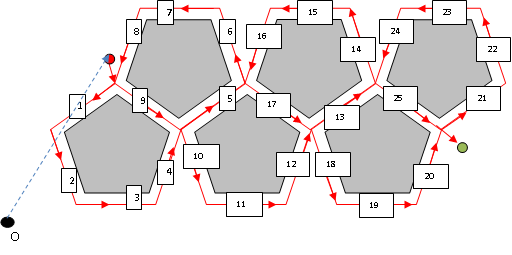
\includegraphics[width=0.95\textwidth]{pentagons.png}
  \caption{Пример составного сегмента резки, содержащего 6 контуров (деталей)}
  \label{fig:ccp-6x5}
\end{figure}

Для включения этих техник в исследование,
понятие контура детали было обобщено
\cite{bib:petunin-2019}
и расширено до
\textit{сегмента резки},
см. Определение~\ref{def:cutting-segment}.

Фактически, пример мультиконтурной резки на~рис.~\ref{fig:ccp-6x5}
также может представлять собой один единственный
сегмент резки в составе некоторой большой задачи.

Ввиду того,
что сегмент резки по определению содержит в себе
направление резки
(от точки врезки $M$ до точки выключения инструмента $M^*$),
нам потребуется ещё более общее понятие:

\begin{opred}
  \textbf{Базовый сегмент резки}
  $B^S$
  ---
  это часть сегмента резки
  $S = \overrightarrow{M M^*}$
  без участков входа и выхода
  (lead-in и lead-out).
\end{opred}

Базовый сегмент содержит только геометрию
(части) контуров, подлежащих резке,
и не содержит информации о направлении резки.

При помощи понятия базового сегмента
формулируется обобщение задачи непрерывной резки:

\textit{Задача непрерывной сегментной резки}
(Segment Continuous Cutting Problem, $SCCP$)
--- это задача резки
для фиксированного набора базовых сегментов резки:
$SCCP = \left\{B^{S_i}\right\}$.

Описанный в данной главе алгоритм,
разработанный для решения задачи непрерывной резки,
естественным образом обобщается на решение
задачи непрерывной сегментной резки.

\begin{figure}
  \centering
  \subfloat[Стандартная резка, 45 сегментов]{
    \label{fig:ccp-gsccp-nest}
    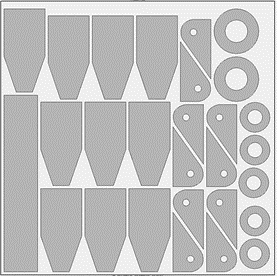
\includegraphics[width=0.45\columnwidth]{nest45.png}
  }
  \subfloat[Мульти-контурная резка, 39 сегментов]{
    \label{fig:ccp-gsccp-multi}
    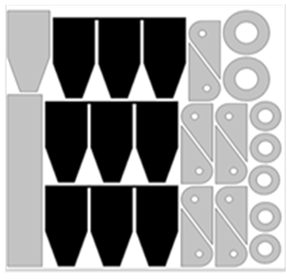
\includegraphics[width=0.47\columnwidth]{nest39.png}
  }
  \caption{Ансамбль задач сегментной резки}
  \label{fig:ccp-gsccp}
\end{figure}

Далее, для произвольного раскройного плана
(то есть фиксированного расположения деталей $A_i$
и контуров $C_i$ на листе $\mathcal B$),
в общем случае можно сгенерировать целый
\textit{ансамбль}
наборов базовых сегментов $B^{S_i}$,
отвечающих заданным контурам деталей $C_i$.
Например,
для раскроя
на рис.~\ref{fig:ccp-gsccp-nest}
можно построить задачу $SCCP$
меньшего размера за счёт
объединения некоторых контуров в базовые сегменты,
как показано на рис.~\ref{fig:ccp-gsccp-multi}.
Это наблюдение приводит нас к ещё более общей задаче резки:

\textit{Обобщённая задача непрерывной сегментной резки}
(Generalized Segment Continuous Cutting Problem, $GSCCP$)
--- это ансамбль из нескольких задач
$SCCP$,
полученных из одного раскройного плана:
$GSCCP = \left\{ SCCP_i \right\}$.

Новые классы
$SCCP$ и $GSCCP$
значительно расширяют существующую классификацию
задач резки для машин термической резки с ЧПУ.
Фактически они представляют собой подклассы
наиболее общей задачи $ICP$,
состоящие из конечного набора базовых сегментов резки.
$$
CCP \subset SCCP \subset GSCCP \subset ICP
$$

\subsection{Общая схема решения задачи GSCCP}

Считая заданным ансамбль
$\left\{ SCCP_i \right\}$
наборов базовых сегментов
$SCCP_i = \left\{B^{S_j}\right\}$,
$
i \in \overline{1, T},
j \in \overline{1, K_i}
$,
будем решать задачу $GSCCP$
следующим образом:

\begin{itemize}
  \item
  Каждая задача
  $SCCP_i$
  решается независимо одним из существующих алгоритмов, например:
  \begin{itemize}
    \item
    Описанный выше эвристический алгоритм решения задачи непрерывной резки,
    см.~Главу~\ref{ch:ccp}.
    \item
    Алгоритм ветвей и границ для обобщённой задачи коммивояжера
    с ограничениями предшествования,
    см.~Главу~\ref{ch:pcgtsp}.
    \item
    Алгоритм на основе динамического программирования,
    дающий точное решение для задач ограниченного размера,
    см.~\cite{bi:RoMa}.
    \item
    Итеративный жадный эвристический алгоритм,
    см.~\cite{bi:greedy}
    \item \dots
  \end{itemize}
  Для дискретных алгоритмов предварительно проводится
  дискретизация контуров и построение конечного
  множества допустимых точек врезки.
  \item
  Выбирается лучшее решение,
  минимизирующее целевую функцию~\eqref{eq:air-move-length}.
\end{itemize}

\begin{figure}
  \centering
  \subfloat[Стандартная резка]{
    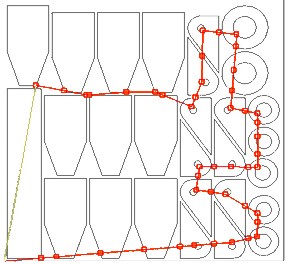
\includegraphics[width=0.45\columnwidth]{cut45.png}
  }
  \subfloat[Мульти-контурная резка]{
    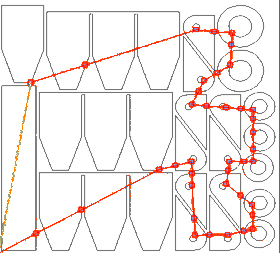
\includegraphics[width=0.47\columnwidth]{cut39.png}
  }
  \caption{Решение задачи GSCCP на рис.~\ref{fig:ccp-gsccp}}
  \label{fig:ccp-gsccp-solution}
\end{figure}

Пример решения задачи $GSCCP$,
представленной на~рис.~\ref{fig:ccp-gsccp},
приведён на~рис.~\ref{fig:ccp-gsccp-solution}.
Использован алгоритм решения задачи непрерывной резки
(без применения дискретизации контуров деталей).
Видно, что для разных постановок задач $SCCP$
действительно получаются разные маршруты
движения режущего инструмента.
Более того,
на практике различие
оказывается ещё более значительным,
поскольку получаемые решения отличаются
также количеством точек врезки,
а эта операция обычно вносит существенные расходы,
как в смысле стоимости резки,
так и затрачиваемого времени.
